\documentclass{article}
\usepackage[T1]{fontenc}
\usepackage{lmodern}
\usepackage{graphicx}
\usepackage{amsmath,amssymb}
\usepackage[a4paper,margin=2cm]{geometry}
\usepackage[absolute,overlay]{textpos}
\setlength{\TPHorizModule}{1mm}
\setlength{\TPVertModule}{1mm}
\usepackage[indonesian]{babel}
\usepackage{hyperref}
\setlength{\emergencystretch}{2em}
% unit: Halaman 19

\begin{document}

% === Halaman 19 (python/native) ===

• Contoh: 

19

P+P = 2P

Sumber gambar: Debdeep Mukhopadhyay, Elliptic Curve Cryptography ,

 Dept of Computer Sc and Engg IIT Madras

𝑚= 𝑑𝑦

𝑑𝑥= 3𝑥𝑝2 + 𝑎

2𝑦𝑝

Koordinat Titik R: 

     xr = m2 – 2xp

     yr = m(xp – xr) – yp

% deskripsi: gambar native xref 93
\noindent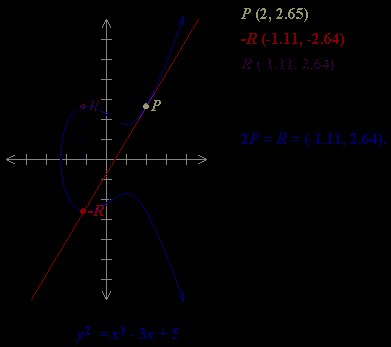
\includegraphics[width=0.85\textwidth]{../../images/python/page_019_img_01.png}

\end{document}
